\RequirePackage{plautopatch}
\documentclass[dvipdfmx,a4paper]{jsarticle}
\usepackage{graphicx}

\usepackage{amsmath}
\usepackage{amssymb}
\usepackage{float}
\usepackage{tikz}
\usepackage{pgfplots}
\pgfplotsset{compat=1.18}

\title{構造力学 課題}
\author{古賀 光一朗}
\date{2025年8月1日}

\begin{document}
\maketitle
\section{課題6}
図に示す幅が$b$で深さが$h$の矩形断面を持つ長さ$l$の梁を考える.この梁が両端(点A,C)で固着され,中央の点Bにおいて単位長さ辺りの大きさが$\omega$の等分布荷重を受ける.また,梁の降伏応力を$\sigma_Y$とする.以下の問いに答えよ.
\begin{enumerate}
    \item 矩形断面の断面2次モーメント$I$および断面係数$Z$を求めよ.
    \item 梁の弾性状態での曲げモーメントの分布を描け.
    \item 矩形断面の全塑性モーメント$M_p$と塑性断面係数$Z_p$を求めよ.
    \item 梁の塑性崩壊時の等分布荷重$\omega_p$を$M_p$を用いて表せ.
    \item 梁の塑性崩壊時の曲げモーメントの分布を描け.
\end{enumerate}

\subsection{矩形断面の断面2次モーメント$I$および断面係数$Z$を求めよ.}

\begin{equation}
    I=\int_A y^2\ dA
    =\int_{-\frac{h}{2}}^{\frac{h}{2}} y^2 \cdot b\ dy=\frac{bh^3}{12}
\end{equation}
よって
\begin{equation}
    Z=\frac{bh^3}{12} \frac{2}{h}=\frac{bh^2}{6}
\end{equation}

\subsection{梁の弾性状態での曲げモーメントの分布を描け.}

力のつりあいの関係より
\begin{equation}
    R_A+R_C=2R
\end{equation}
\begin{equation}
    \therefore\ R=\frac{\omega l}{2}
\end{equation}
モーメントのつりあいの関係より
\begin{equation}
    M_A-M_C-\frac{\omega l^2}{2}+Rl=0    
\end{equation}
\begin{equation}
    \Rightarrow M_A-M_C-\frac{\omega l^2}{2}+Rl=0
\end{equation}
\begin{equation}
    \Rightarrow M_A=M_C
\end{equation}
A端から距離$x$の点で仮想断面をとると\\
\begin{equation}
    M(x)=-M_A+\frac{\omega l}{2}x-\frac{\omega x^2}{2}
\end{equation}
\begin{equation}
    EIy''=M(x)=-M_A+\frac{\omega l}{2}x-\frac{\omega x^2}{2}
\end{equation}
\begin{equation}
    EIy'=-M_Ax+\frac{\omega l}{4}x^2-\frac{\omega}{6}x^3+C_1
\end{equation}
\begin{equation}
    EIy=-\frac{1}{2}M_Ax^2+\frac{\omega l}{12}x^3-\frac{\omega}{24}x^4+C_1x+C_2
\end{equation}
$x=0$で$y'=0$, $y=0$なので
\begin{equation}
    C_1=C_2=0
\end{equation}
$x=\frac{l}{2}$で$y'=0$なので
\begin{equation}
    M_A=\frac{\omega l^2}{12}
\end{equation}
\begin{equation}
\begin{aligned}
    M(x)&=\frac{\omega}{2}x^2-\frac{\omega l}{2}x-\frac{\omega l^2}{12}\\
    &=-\frac{\omega}{2}(x-\frac{l}{2})^2+\frac{\omega l^2}{24}\\
\end{aligned}
\end{equation}

\vspace{1cm}

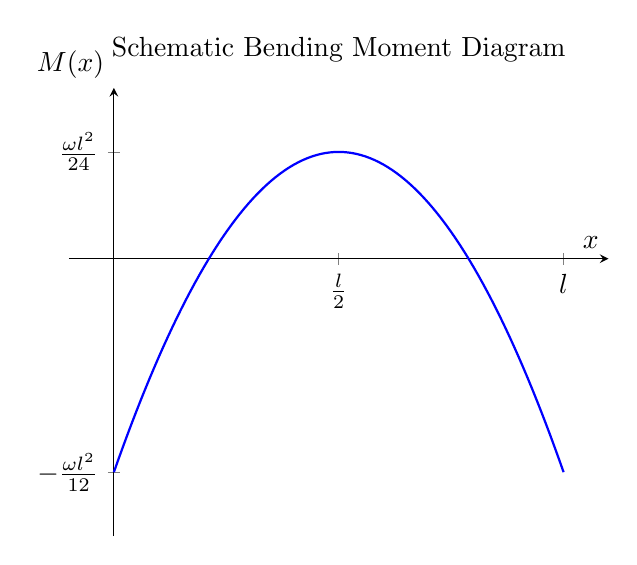
\begin{tikzpicture}

    \def\myL{12}
    \def\myomega{2}

    \pgfmathsetmacro{\Mend}{-\myomega*\myL*\myL/12}
    \pgfmathsetmacro{\Mmax}{\myomega*\myL*\myL/24}

    \begin{axis}[
        title={Schematic Bending Moment Diagram},
        axis lines=middle,
        xlabel={$x$},
        ylabel={$M(x)$},
        ylabel style={anchor=south east},
        xtick={0, \myL/2, \myL},
        xticklabels={{$0$}, {$\frac{l}{2}$}, {$l$}},
        ytick={\Mend, \Mmax},
        yticklabels={{$-\frac{\omega l^2}{12}$}, {$\frac{\omega l^2}{24}$}},
        domain=0:\myL,
        samples=101,
        enlarge x limits=0.1,
        enlarge y limits=0.2
    ]

        % --- 【最終修正点】ここの「^2」を掛け算に変更 ---
        \addplot[blue, thick] {-\myomega/2 * (x - \myL/2)*(x - \myL/2) + \myomega*\myL*\myL/24};

    \end{axis}

\end{tikzpicture}





\subsection{矩形断面の全塑性モーメント$M_p$と塑性断面係数$Z_p$を求めよ.}

\begin{equation}
    M_p=(\sigma_Y \cdot b \cdot \frac{h}{2}) \times(\frac{h}{2})=\frac{\sigma_Y bh^2}{4}
\end{equation}
\begin{equation}
    Z_p=\frac{bh^2}{4}
\end{equation}

\subsection{梁の塑性崩壊時の等分布荷重$\omega_p$を$M_p$を用いて表せ.}

\begin{equation}
\begin{aligned}
    M(x) &= -M_P+\frac{\omega_p l}{2}x-\frac{\omega_p}{2}x^2\\
    &=-\frac{\omega_p}{2}(x-\frac{l}{2})^2-M_p+\frac{\omega_p l^2}{8}\\
    &=-\frac{\omega_p}{2}(x-\frac{l}{2})^2+M_p
\end{aligned}
\end{equation}
よって
\begin{equation}
    \omega_p = \frac{16M_p}{l^2}
\end{equation}

\subsection{梁の塑性崩壊時の曲げモーメントの分布を描け.}

\begin{equation}
\begin{aligned}
  M(x) &= -M_p+\frac{\omega_p l}{2}x-\frac{\omega_p}{2}x^2 \\
       &= -\frac{\omega_p}{2}(x-\frac{l}{2})^2-M_p+\frac{\omega_p l^2}{8}
\end{aligned}
\end{equation}
\vspace{1cm}

\begin{tikzpicture}
\centering

    % --- Step 1: 計算に使うための「変数」を定義 ---
    \def\myL{12}
    \def\myomegap{2}
    \def\myMp{30}

    % --- Step 2: y軸の目盛りの「場所」を計算 ---
    \pgfmathsetmacro{\Mend}{-\myMp}
    \pgfmathsetmacro{\Mmax}{-\myMp + \myomegap*\myL*\myL/8}

    % --- Step 3: 軸とグラフを描く本体 ---
    \begin{axis}[
        title={$M(x) = -\frac{\omega_p}{2}(x-\frac{l}{2})^2-M_p+\frac{\omega_p l^2}{8}$},
        axis lines=middle,
        xlabel={$x$},
        ylabel={$M(x)$},
        ylabel style={anchor=south east},
        xtick={0, \myL/2, \myL},
        xticklabels={{$0$}, {$\frac{l}{2}$}, {$l$}},
        ytick={\Mend, \Mmax},
        yticklabels={{$-M_p$}, {$-M_p + \frac{\omega_p l^2}{8}$}},
        domain=0:\myL,
        samples=101,
        enlarge x limits=0.1,
        enlarge y limits=0.2
    ]

        % --- 【最終修正】数式の定数部分を、計算済みの「\Mmax」に置き換え ---
        \addplot[blue, thick] {-\myomegap/2 * (x - \myL/2)*(x - \myL/2) + \Mmax};

    \end{axis}

\end{tikzpicture}


\end{document}